\documentclass[10pt,a4paper]{article}
\renewcommand{\familydefault}{\sfdefault}
\usepackage[left=3cm, right=3cm, top=2cm, bottom=2cm, textwidth=15cm]{geometry}
\usepackage[utf8]{inputenc}
\usepackage[T1]{fontenc}
\usepackage[english]{babel}
\usepackage{graphicx}
\usepackage{xfrac}
\usepackage{sectsty}
\usepackage{hyperref}
\sectionfont{\rmfamily\selectfont}
\usepackage{ccicons}

\begin{document}
\thispagestyle{empty}
\pagenumbering{gobble}
\title{Recipe book\\
	\vspace{1cm}
	{\large Project as part of the training in system catering}\\
	{\small 1st year vocational school}
	\vspace{2cm}
}
\author{Lisa Machoi}
\date{\today}
\maketitle
\newpage
\thispagestyle{empty}
\tableofcontents
\setcounter{page}{0}
\pagenumbering{arabic}
%
\newpage
\setcounter{page}{1}
\section{\textsc{Side salad}}

\subsection*{Ingredients for 2 portions:}

\begin{tabular}{p{7.5cm} p{7.5cm}}
	& \\
	4leafs oak leaf lettuce & \sfrac{1}{2} cucumber \\
	2 carrots & \sfrac{1}{4} radish
\end{tabular}

\subsection*{Serving suggestion:}

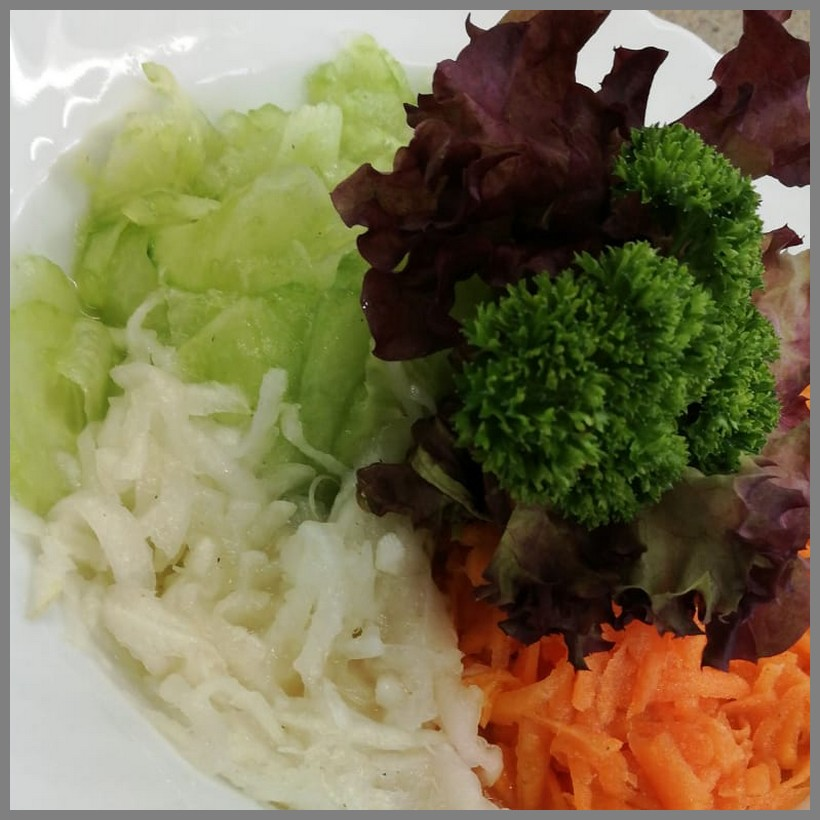
\includegraphics[width=\textwidth]{img/beilagensalat.jpeg} \cite{beilagensalat}

\subsection*{How it's done:}
\begin{tabular}{p{15cm}}
	\\
	Coarsely grate the radish, carrots and julienne the cucumber.\\
	Dress the salad on a plate.
\end{tabular}

\section{Rohkostsalat mit Apfel}

\textbf{Zutaten für 4 Personen:}
\begin{itemize}
  \item 1x Weißkohlkopf
  \item 4x Karotten
  \item 2x Äpfel
  \item 6EL Olivenöl
  \item 6EL Weißweinessig
  \item 2EL Salz
  \item Pfeffer, Zucker, Kümmel nach Geschmack
\end{itemize}

\textbf{Zubereitung:}
\begin{itemize}
  \item Den Weißkohl teilen und danach in dünne Streifen schneiden.
  \item Wir empfehlen hier die Schnittform Julienne.
  \item Danach die Äpfel und die Karotten schälen.
  \item Den Apfel in Achtel teilen.
  \item Salz und Essig hinzufügen und solange fest kneten, bis der Kohl einen eigenen Saft bildet.
  \item Nun mit Pfeffer, Zucker und den anderen Gewürzen abschmecken.
  \item Danach das Gemisch einige Zeit ziehen lassen und fertig ist der Rohkostsalat.
\end{itemize}

Coleslaw Salad

ingredients:	1		half cabbage
		1		carrot
		1		onion
		65 gram	sugar
½ ts.		salt
		½ ts.		pepper
		½ cup		milk
		125gram	mayonnaise
		½ cup		buttermilk
		4 ts.		 white wine vinegar
		6 ts.		lemon juice
		2 ts.		paprika
		2 ts.		mustard

Cut the cabbage, the carrot and the onion in small strips (= Julienne).
Now you mix the vegetables in a big bowl.
After that you put the other ingredient into another bowl and mix it too.
You put the dressing over the mix of the vegetables.

Let the mixture pass for eight to ten hours.

Before you serve it, stir it a little bit.

Enjoy your salad!

\section{\textsc{Schneller Gurkensalat mit saurer Sahne und Dill}}

\subsection*{Zutaten:}

\begin{tabular}{p{7.5cm} p{7.5cm}}
	& \\
	1 Salatgurke & 1 Becher Saure Sahne \\
	1 TL Gehackter Dill & Salz, Pfeffer
\end{tabular}

\subsection*{Serviervorschlag:}


\includegraphics[width=\textwidth]{img/ph.jpg} \cite{gurkensalatdill}

\subsection*{So geht's:}

\begin{tabular}{p{15cm}}
	\\
  Die Gurke in dünne Scheiben schneiden, oder mit einer Küchenreibe reiben.\\
  Zusammen mit der sauren Sahne in eine Schüssel geben.\\
  Mit Salz und Pfeffer abschmecken.\\
  Frisch und gekühlt servieren.
\end{tabular}

\section{\textsc{Cucumber salad}}

\subsection*{Zutaten für 2 Portionen:}

\begin{tabular}{p{7.5cm} p{7.5cm}}
	& \\
	\sfrac{1}{2} cucumber & 2tbsp olive oil \\
	1tbsp vinegar & 1tbsp sugar \\
	\multicolumn{2}{l}{salt, papper, dill to taste}
\end{tabular}

\subsection*{Serving recommendation:}

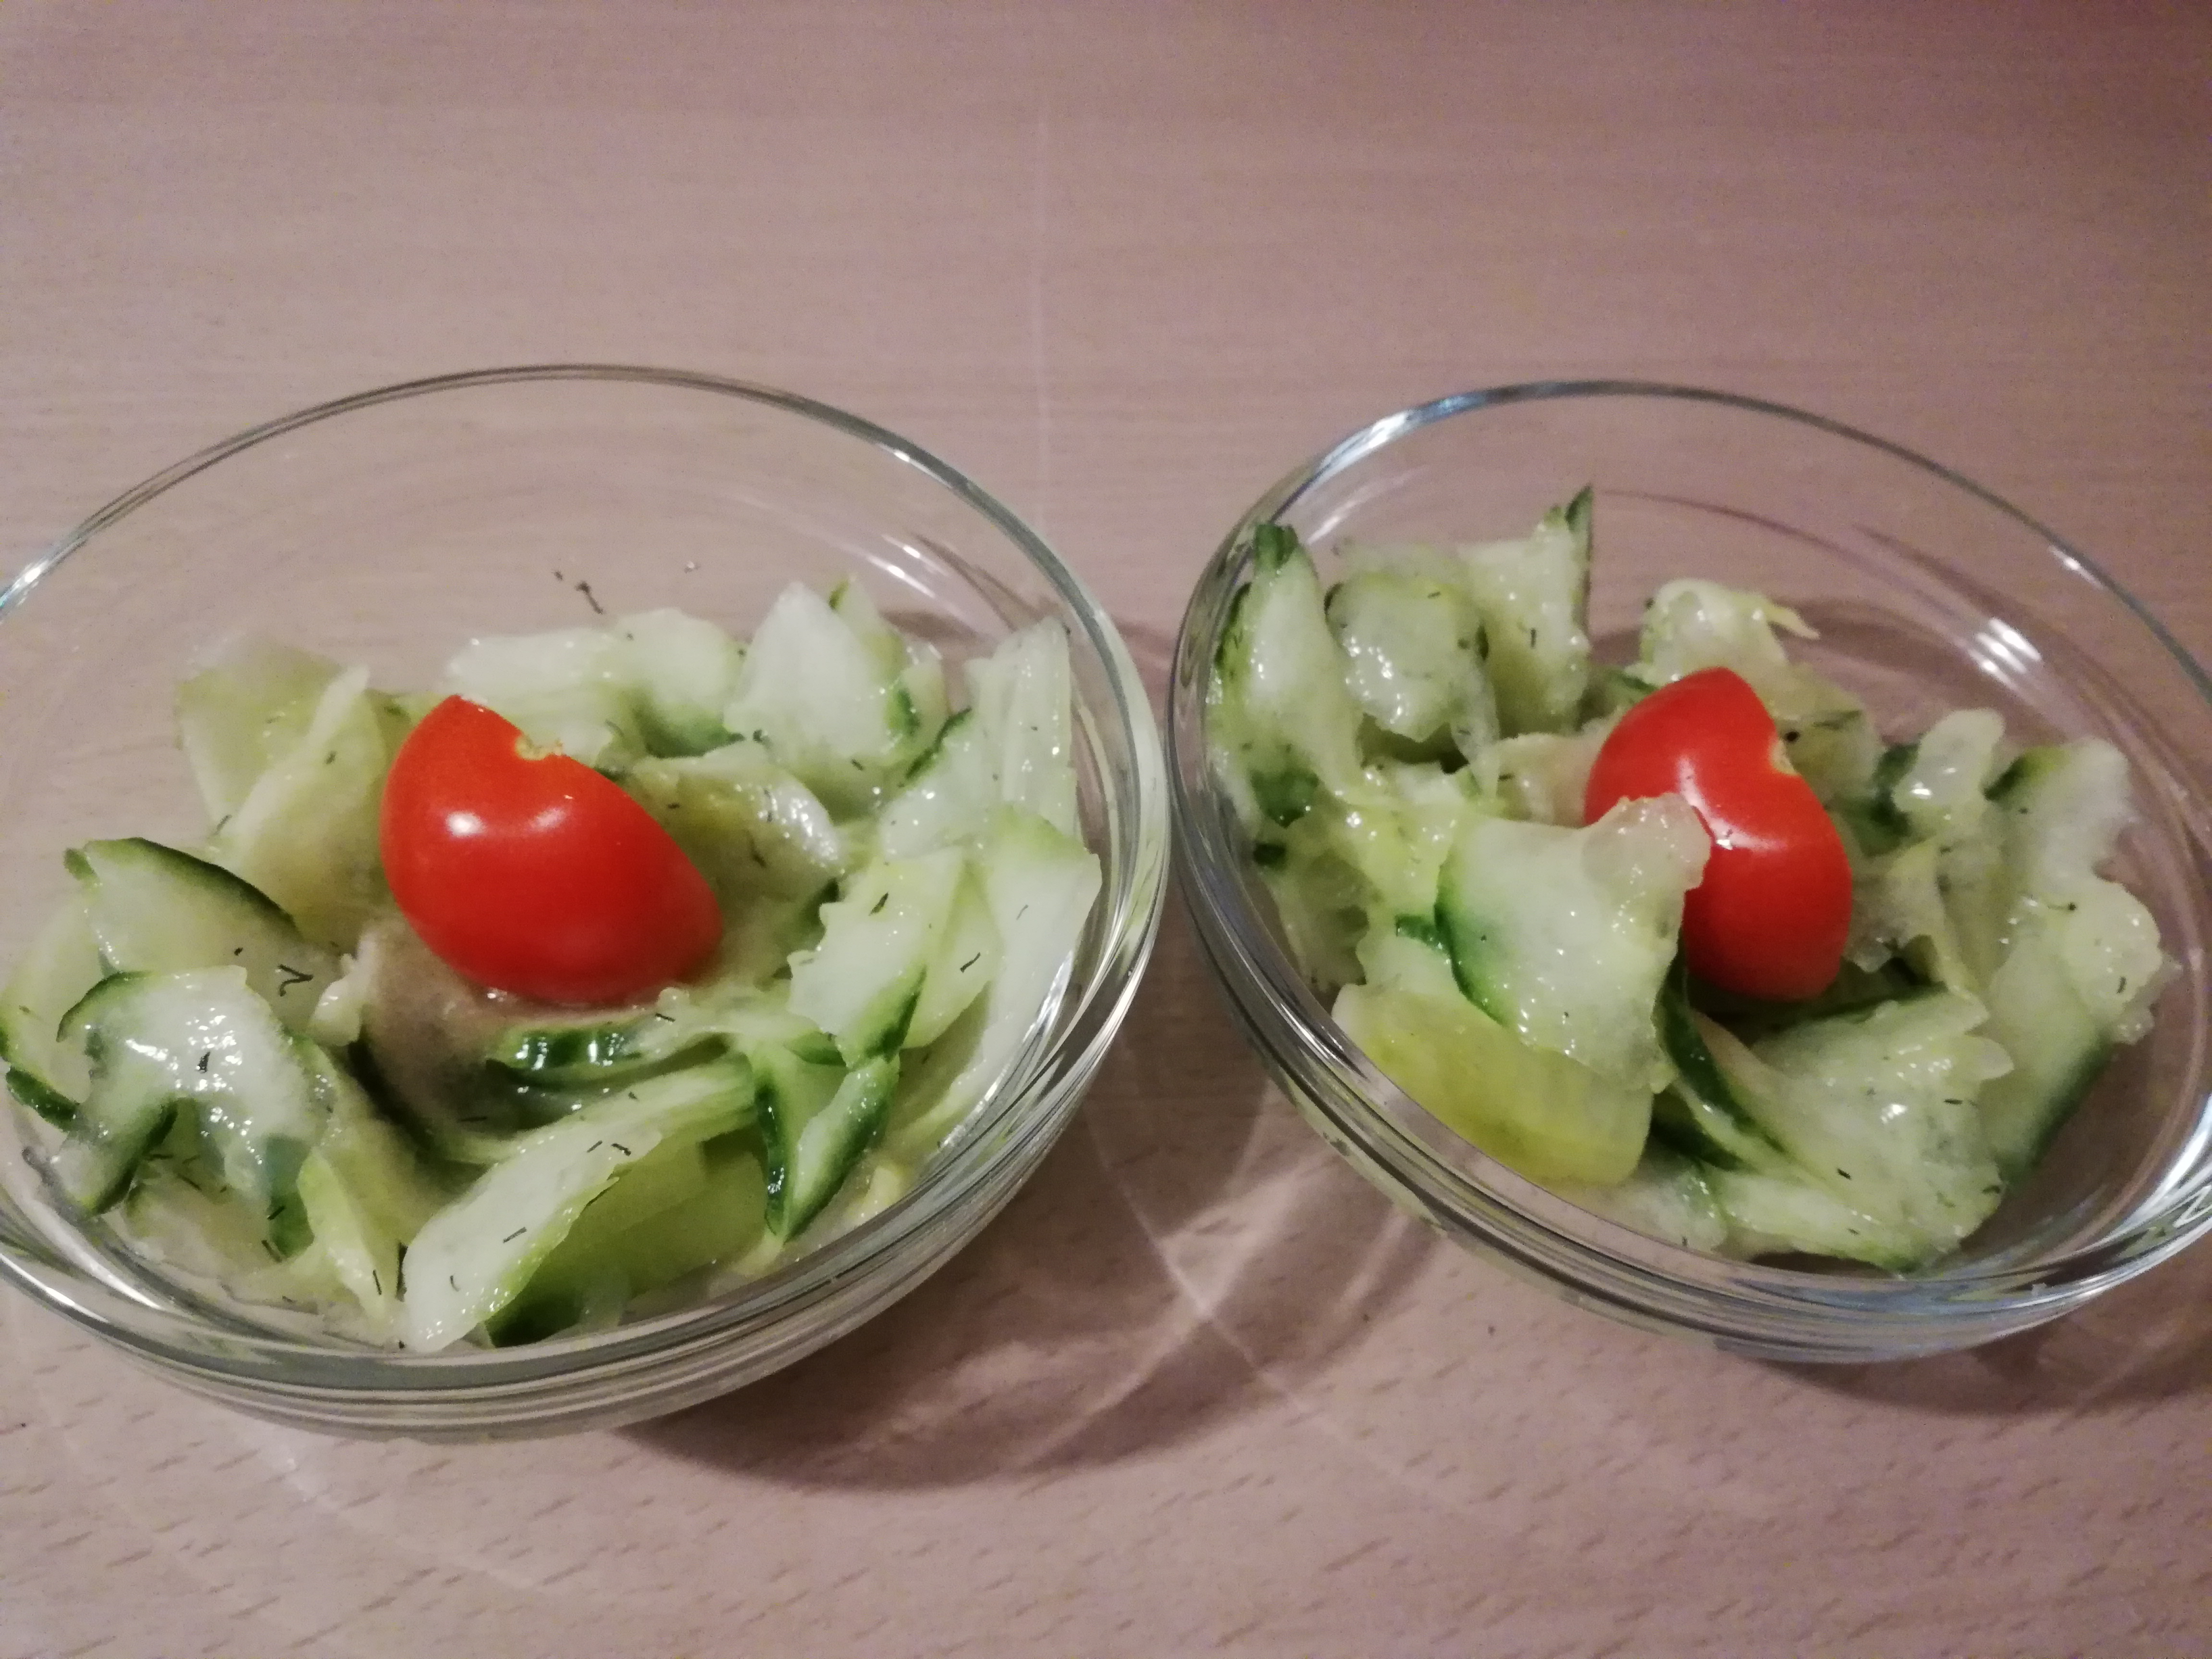
\includegraphics[width=\textwidth]{img/gurkensalat/gurkensalat_fertig.jpg} \cite{gurkensalat}

\subsection*{How it's done:}

\begin{tabular}{p{15cm}}
	\\
  Partially peel half of the cucumber with a peeler.\\
  This creates a dash of colour in the finished salad.\\
  Add the spices and oils and leave to stand for about 2 hours.
\end{tabular}


Spring egg salad
Ingredients for 2 people:

For the sauce:
- 2 hard-boiled eggs
- 1 clove of garlic
- 1 shallot
- 1 tsp mustard
- 3 tbsp vinegar
- 4 tbsp olive oil
- 5 tablespoons fresh herbs (e. g. chives, parsley, basil)
- salt/pepper

For the salad:
- Various leaf salads (e. g. iceberg lettuce, lamb's lettuce)
- 1 tsp vinegar
- salt/pepper
- 1l olive oil
- 4 hard-boiled eggs


1. cut the eggs in half and separate the egg yolk from the egg white. Peel and chop the garlic and shallots.
2. place the egg yolk, mustard, garlic and shallots in a measuring cup.
3. add the vinegar and oil and leave to stand for a few minutes.
In the meantime, finely chop the herbs with a chopping knife. And add it to the other ingredients.
5. throw the egg whites in small cubes and add to the mixture.
6. puree finely and season to taste.
7. clean and chop the salads.
8. add oil, vinegar and spices and leave to stand for 10 minutes.
9. arrange in a large bowl and garnish with the remaining egg.
Serve with 10 baguettes or fresh rolls.

tip

The salad makes itself super at Easter time. There are often boiled eggs left, which can be processed so well.

\section{\textsc{Omlett}}

\subsection*{Zutaten:}

\begin{tabular}{p{7.5cm} p{7.5cm}}
	& \\
	6 Eier & 40g Butter \\
	20ml Wasser & 20ml Milch \\
  1TL Salt & Pfeffer, Salz \& Muskat \\
  Schnittlauch zum Garnieren &
\end{tabular}

\subsection*{Serviervorschlag:}


\includegraphics[width=\textwidth]{img/ph.jpg} \cite{omlett}

\subsection*{So geht's:}

\begin{tabular}{p{15cm}}
	\\
  Die Eier aufschlagen und in eine Schüssel geben.\\
  Mit den Gewürzen nach Geschmack würzen und mit Wasser und Milch aufschlagen. \\
  Die Masse in eine heiße Pfanne geben. Nach und nach stocken lassen.\\
  Zusammenklappen und mit Butter bestreichen. 
\end{tabular}


“Whipped"; omelet

Ingredients for 1 omelette:
4 eggs
2 Vienna sausages
1x half onion
200g Mozzarella
salt, pepper

Preparation

Beat the eggs in a bowl until foamy.
Melt the butter in a large pan.
In the meantime, cut the Wiener into thin slices.
Finely dice the onions.
Pour the egg mixture into the pan and let it set over a high heat.
Spread the Wiener and the onions over the omelette.
Fry with a lid on the pan for 5 minutes.
Serve on a large plate.

\section{\textsc{Omelette tomo}}

\subsection*{Ingredients for 1 omelette:}

\begin{tabular}{p{7.5cm} p{7.5cm}}
	& \\
	4 eggs & 5 Cherrytomatoes \\
	2ts butter & 200g mozzarella \\
	salt & pepper \\
	basil to taste &
\end{tabular}

\subsection*{Serving suggestion:}

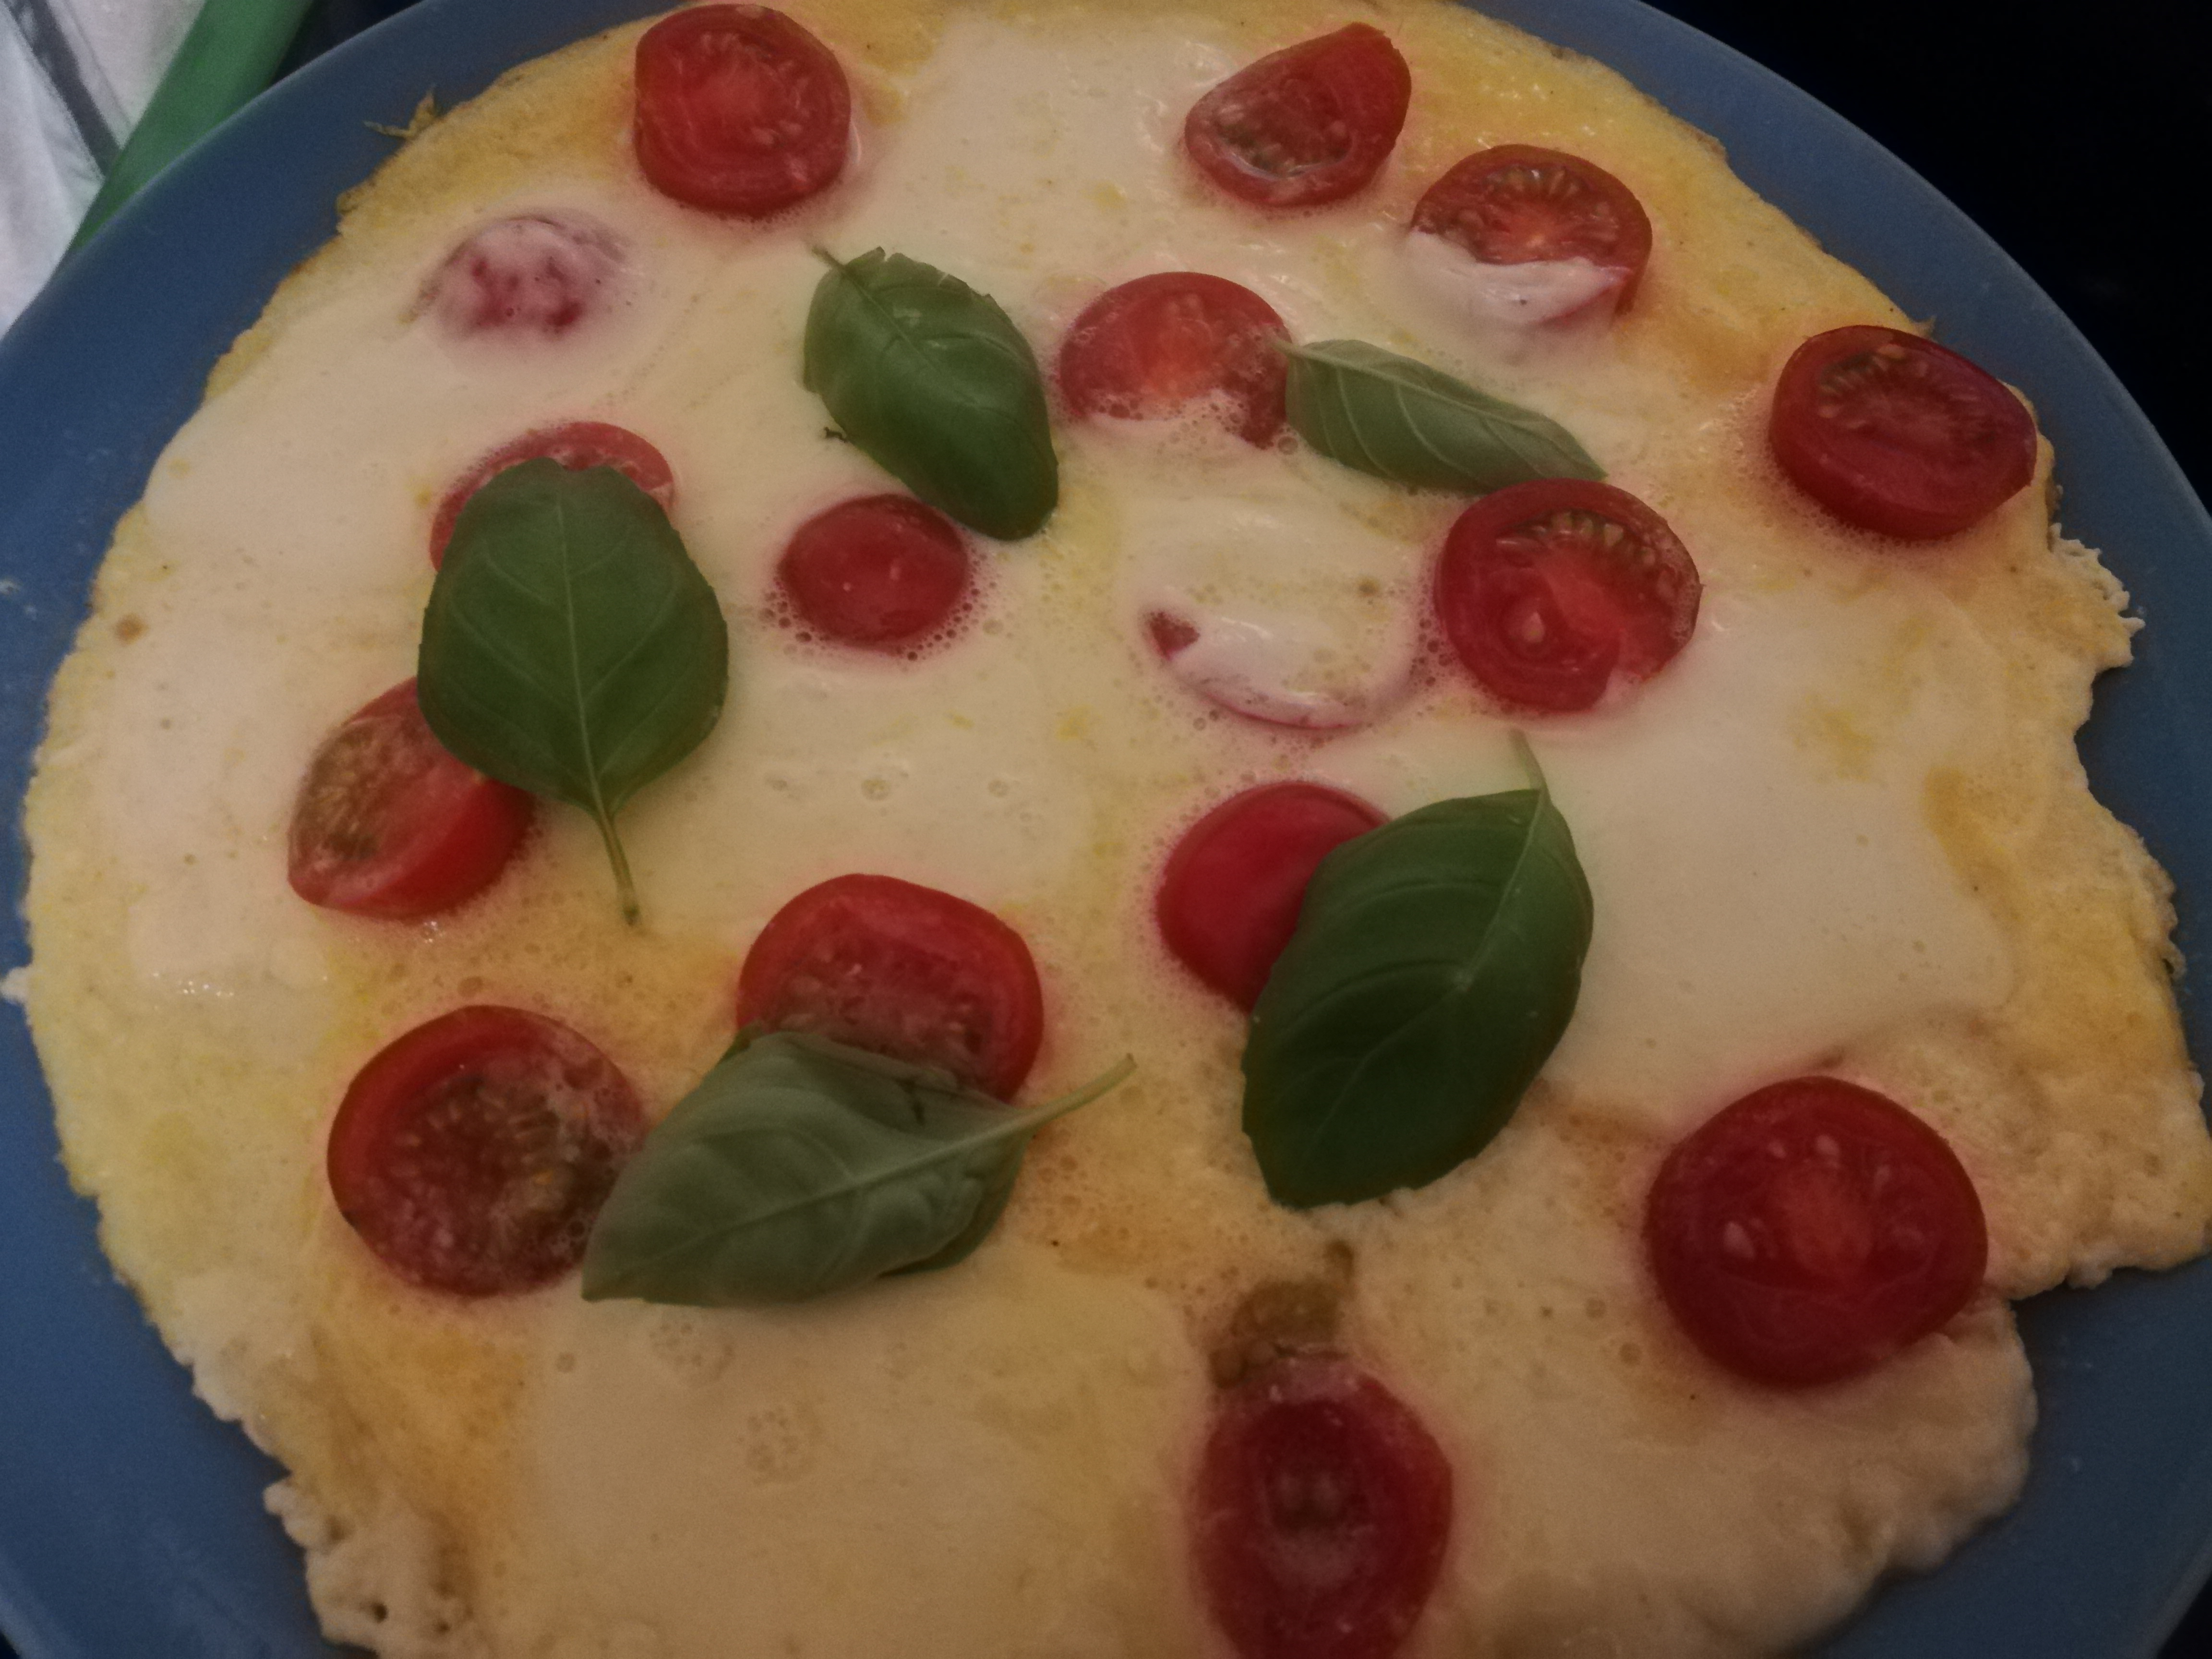
\includegraphics[width=\textwidth]{img/omlett/omlett_tomo_fertig.jpg} \cite{omlettomo}

\subsection*{How it's done:}

\begin{tabular}{p{15cm}}
	\\
  Beat the eggs with a whisk until it is foamy.\\
  Add salt and pepper to taste.\\
  Melt the butter in a pan.\\
  Pour the egg mixture into the pan and let it set over a high heat.\\
  Spread the mozzarella and the tomatoes on it.\\
  Fry with a lid on a low heat for 5 minutes.\\
  Place it on a large plate and decorate it with basil.
\end{tabular}

\section{\textsc{Italian fried eggs}}

\subsection*{Ingredients:}

\begin{tabular}{p{7.5cm} p{7.5cm}}
	& \\
	6 eggs & mozzarella \\
	oil for the pan & Spices to taste
\end{tabular}

\subsection*{Serving suggestion:}


\includegraphics[width=\textwidth]{img/ph.jpg} \cite{itaspiegelei}

\subsection*{How it's done:}

\begin{tabular}{p{15cm}}
	\\
  Heat the oil in the pan.\\
  Cut the tomato into thin slices and sauté in a pan.\\
  Now beat the eggs in the pan.\\
  As soon as it begins to falter, spread the mozzarella evenly over it.\\
  Season and you're done.
\end{tabular}

\section{\textsc{Italian fried eggs}}

\subsection*{Ingredients for 2 portions:}

\begin{tabular}{p{7.5cm} p{7.5cm}}
	& \\
	6 eggs & mozzarella \\
	oil for the pan & Spices to taste
\end{tabular}

\subsection*{Serving suggestion:}

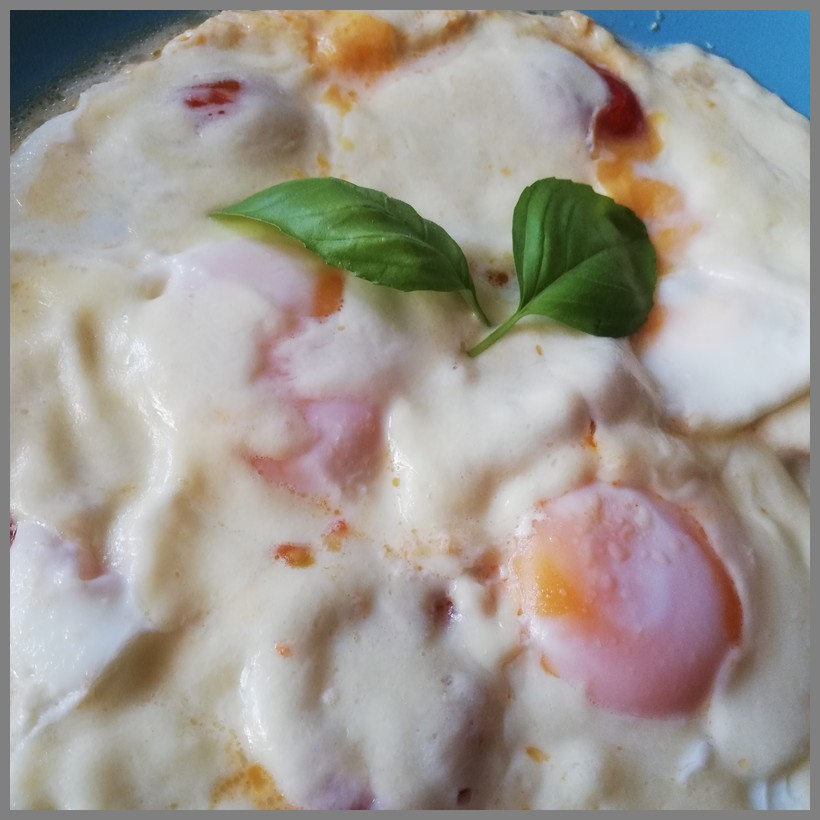
\includegraphics[width=\textwidth]{img/spiegelei_ita.jpg} \cite{itaspiegelei}

\subsection*{How it's done:}

\begin{tabular}{p{15cm}}
	\\
  Heat the oil in the pan.\\
  Cut the tomato into thin slices and sauté in a pan.\\
  Now beat the eggs in the pan.\\
  As soon as it begins to falter, spread the mozzarella evenly over it.\\
  Season and you're done.
\end{tabular}

\section{\textsc{Rührei}}

\subsection*{Zutaten:}

\begin{tabular}{p{7.5cm} p{7.5cm}}
	& \\
	3 Eier & 125ml Milch \\
	1EL Öl & Salz, Pfeffer, Muskatnuss
\end{tabular}

\subsection*{Serviervorschlag:}

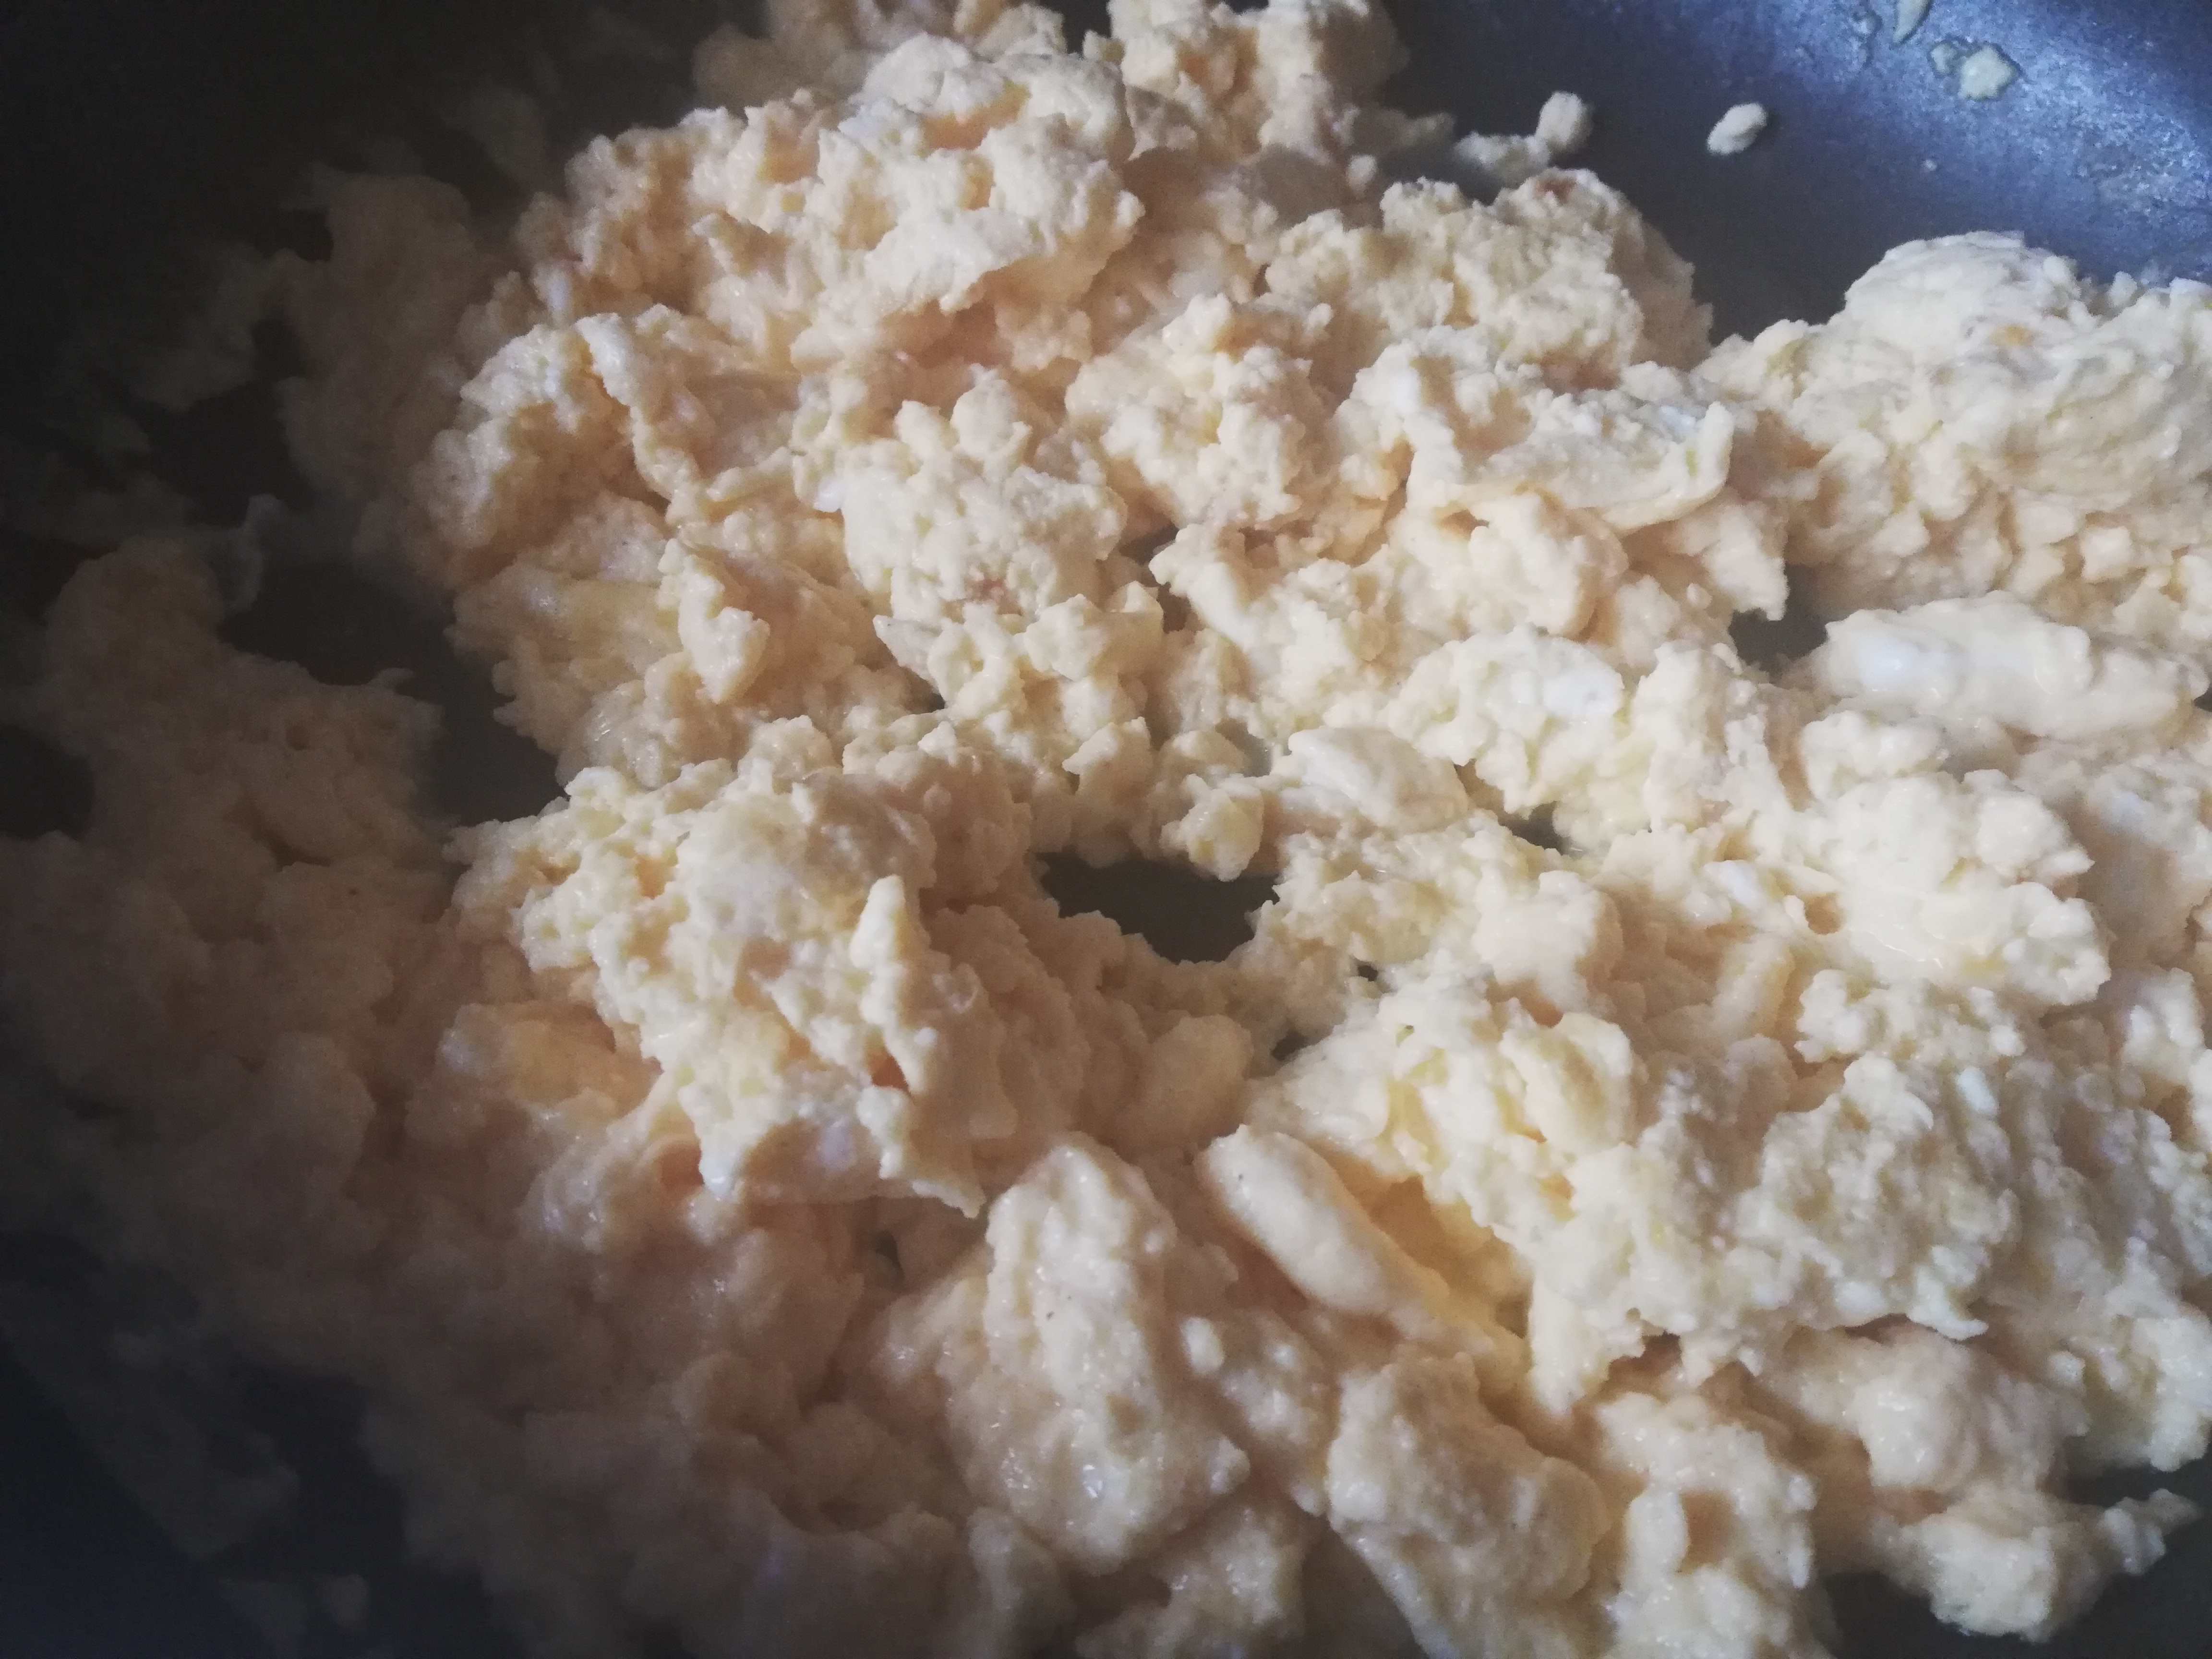
\includegraphics[width=\textwidth]{img/ruehrei/ruehrei_fertig.jpg} \cite{ruehrei}

\subsection*{So geht's:}

\begin{tabular}{p{15cm}}
	\\
	Die Milch in einem Messbecher abfüllen. Die Eier auch in diesen schlagen. Mit einem Schneebesen zu einer glatten Masse rühren.\\
	Je nach Geschmack mit Salz, Pfeffer und Muskatnuss würzen.\\
	Öl in einer Pfanne erhitzen. Die gesamte Eimasse hineingeben.\\
	Kurz stocken lassen. Das Ei nun mit einem Pfannenschaber von innen nach außen schieben. Vorgang so lange wiederholen, bis das gesamte Ei gestockt ist.
\end{tabular}
\section{\textsc{Scrambled eggs on wholemeal rolls}}

\subsection*{Ingredients for 2 portions:}

\begin{tabular}{p{7.5cm} p{7.5cm}}
	& \\
	5 eggs & 2 wholemeal rolls \\
	1 tomato & 20g butter \\
  1tbsp cress & 2 salad leaves \\
  fresh herbs & tartar sauce \\
  oil for the pan & a sip of mineral water \\
  salt, pepper \& nutmeg
\end{tabular}

\subsection*{Serving suggestion:}

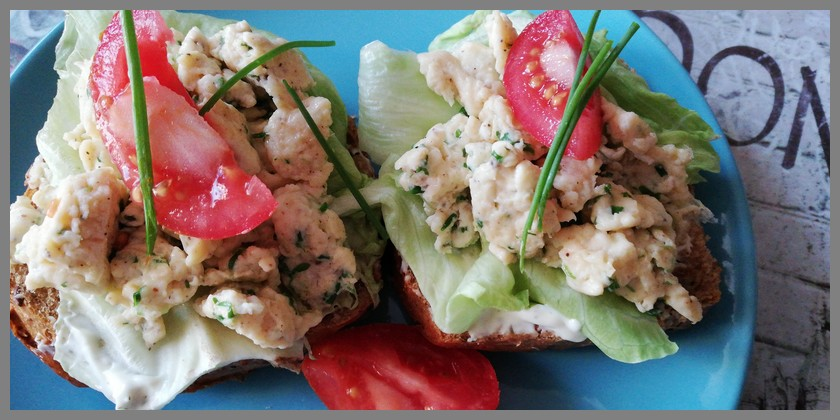
\includegraphics[width=\textwidth]{img/ruehrei_vollkorn.jpeg} \cite{ruehreivollkorn}

\subsection*{How it's done:}

\begin{tabular}{p{15cm}}
	\\
  Mix eggs, herbs and mineral water in a bowl.\\
  Heat the oil in a flat pan. Add the egg mass.\\
  Leave to falter and gradually slide from the outside to the inside with a scraper.\\
  In the meantime, cut the rolls open and coat them with tartar sauce.\\
  Place a salad leaf on top. Spread the scrambled eggs on the salad and garnish with half a tomato.
\end{tabular}

\section{\textsc{French egg in a saucer}}

\subsection*{Ingredients for 2 bowls:}

\begin{tabular}{p{7.5cm} p{7.5cm}}
	& \\
	6tbsp sour cream & 2 eggs \\
	2tbsp fresh, chopped herbs  & 2 cocktail tomatoes \\
  salt, pepper \& nutmeg & baguette as a side dish
\end{tabular}

\subsection*{Serving suggestion:}

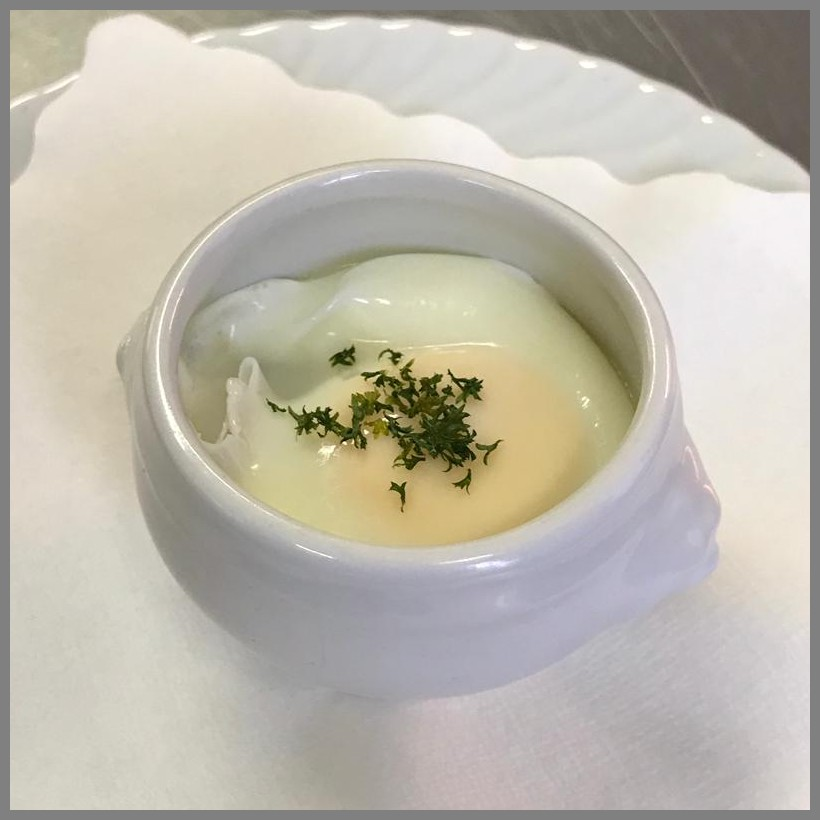
\includegraphics[width=\textwidth]{img/ei_naepfchen.jpg} \cite{eiimnaepfchen}

\subsection*{How it's done:}

\begin{tabular}{p{15cm}}
	\\
  Preheat the oven to 180 degrees.\\
  Mix sour cream with spices and herbs.\\
  Share the mass. Pour the first part into 2 cream andrulee moulds.\\
  Beat one egg each and spread the rest of the cream on top.\\
  Half fill a large casserole dish with water.\\
  Place the moulds in the oven and push them into the oven.\\
  Let simmer for 25 minutes.\\
  Approximately 5 minutes before the end of the time distribute two quartered tomatoes on the bowls.\\
  Take out of the oven and drain on a paper towel. Slice bread and serve.
\end{tabular}

\section{\textsc{French egg in a saucer}}

\subsection*{Ingredients for 2 bowls:}

\begin{tabular}{p{7.5cm} p{7.5cm}}
	& \\
	6tbsp sour cream & 2 eggs \\
	2tbsp fresh, chopped herbs  & 2 cocktail tomatoes \\
  salt, pepper \& nutmeg & baguette as a side dish
\end{tabular}

\subsection*{Serving suggestion:}

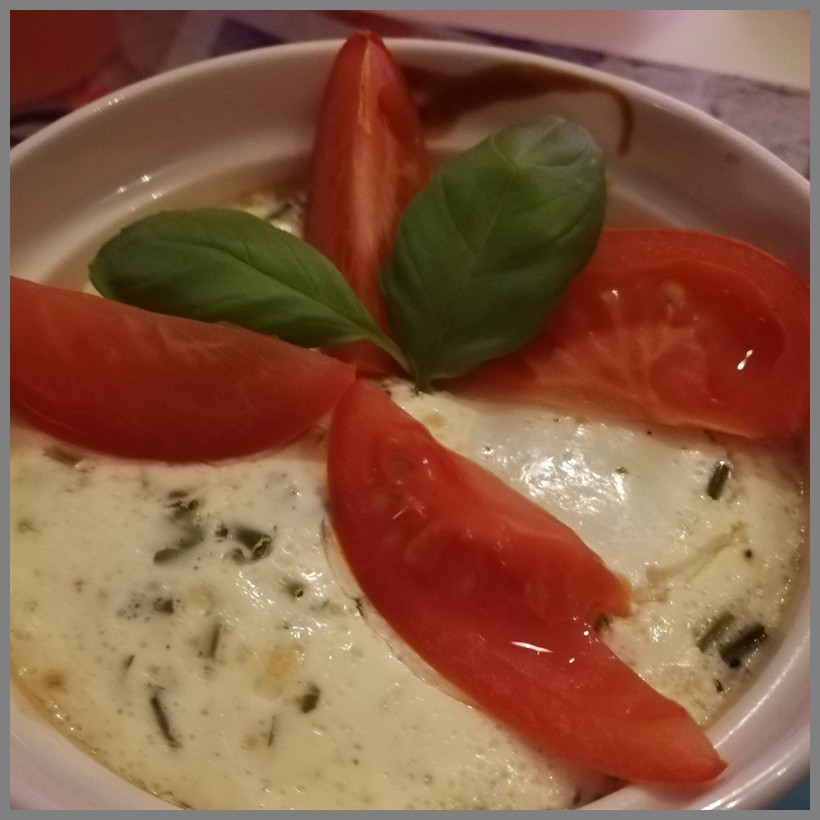
\includegraphics[width=\textwidth]{img/ei_naepfchen_franz.jpg} \cite{eiimnaepfchenfranz}

\subsection*{How it's done:}

\begin{tabular}{p{15cm}}
	\\
  Preheat the oven to 180 degrees.\\
  Mix sour cream with spices and herbs.\\
  Share the mass. Pour the first part into 2 cream andrulee moulds.\\
  Beat one egg each and spread the rest of the cream on top.\\
  Half fill a large casserole dish with water.\\
  Place the moulds in the oven and push them into the oven.\\
  Let simmer for 25 minutes.\\
  Approximately 5 minutes before the end of the time distribute two quartered tomatoes on the bowls.\\
  Take out of the oven and drain on a paper towel. Slice bread and serve.
\end{tabular}

\section{\textsc{Poached egg in mustard sauce}}

\subsection*{Ingredients:}

\begin{tabular}{p{7.5cm} p{7.5cm}}
	& \\
	100g butter & 1 onion \\
	3tbsp flour & 250ml milk \\
  250ml vegetable broth & 4 eggs \\
  2tbsp mustard & 5tbsp vinegar \\
  1,5l water &
\end{tabular}

\subsection*{Serving suggestion:}


\includegraphics[width=\textwidth]{img/ph.jpg} \cite{eisenfsosse}

\subsection*{How it's done:}

\begin{tabular}{p{15cm}}
	\\
  Melt the butter in a saucepan. Cut the onions into small cubes and add to the butter.\\
  Sweat until glassy. Gradually spread the flour on top - let the roux develop.\\
  Add the milk and stir vigorously to prevent lumps from forming. Add the vegetable stock. Simmer slowly.\\
  Bring the water to the boil in a small pot. Add vinegar.\\
  Beat the eggs in a flat cup without damaging the yolk.\\
  Now let it glide quickly but carefully into the boiling water.\\
  Poach for 4-7 minutes according to taste.\\
  Then add the eggs to the mustard sauce and bring to the boil again.\\
  Parsley potatoes or airy mashed potatoes are an excellent accompaniment.
\end{tabular}

\section{\textsc{Spaghetti spinach carbonara with poached egg}}

\subsection*{Ingredients for 2 portions:}

\begin{tabular}{p{7.5cm} p{7.5cm}}
	& \\
	200g spaghetti & 2 handfull fresh spinach \\
	\sfrac{1}{2} diced onion & \sfrac{1}{2} garlic clove \\
  40g bacon & 3 eggs \\
  100ml page & dash of vinegar \\
  salt, pepper & 1tbsp sunflower oil
\end{tabular}

\subsection*{Serving suggestion:}

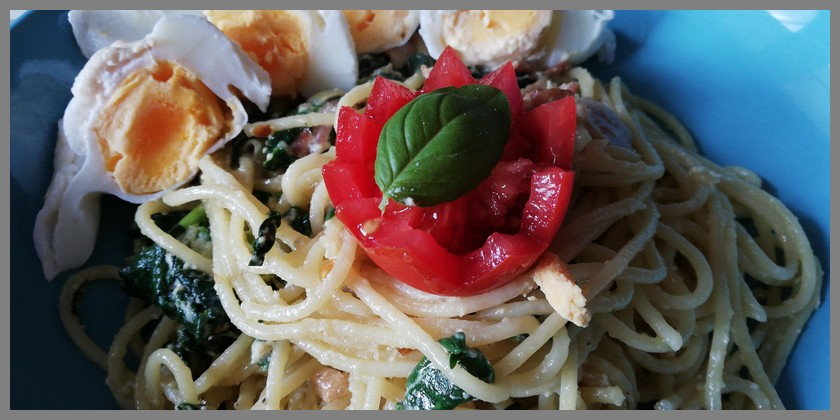
\includegraphics[width=\textwidth]{img/spaghetti_ei.jpeg} \cite{eicorbonara}

\subsection*{How it's done:}

\begin{tabular}{p{15cm}}
	\\
  First cook the spaghetti according to the package instructions al denkte.\\
  Then cut the bacon into 4cm long strips.\\
  Put the oil in a hot pan and fry the onions and bacon until crispy.\\
  After about 5 minutes, add the spinach and fry until it collapses. Season with salt and pepper.\\
  Now add the spaghetti to a larger pan (or roaster).\\
  Pour the cream into a measuring cup and add an egg. Beat both.\\
  Pour over the spinach mix and reduce everything.\\
  In another top bring about 1,5l water to the boil.\\
  Turn down the heat so that the water only boils slightly. Add the vinegar.\\
  Whip an egg in a flat cup. Make sure that the egg yolk remains undamaged.\\
  From the cup, let the egg slide slowly into the hot water. Poach for 6-7 minutes.\\
  Repeat with another egg.
\end{tabular}

\section{\textsc{Egg pancakes}}

\subsection*{Ingredients for 2 portions:}

\begin{tabular}{p{7.5cm} p{7.5cm}}
	& \\
	100g flour & 40g sugar \\
	300ml milk & 4 eggs \\
	pinch of salt & oil for the pan \\
	\multicolumn{2}{l}{Icing sugar for decoration}
\end{tabular}

\subsection*{Serving suggestion:}

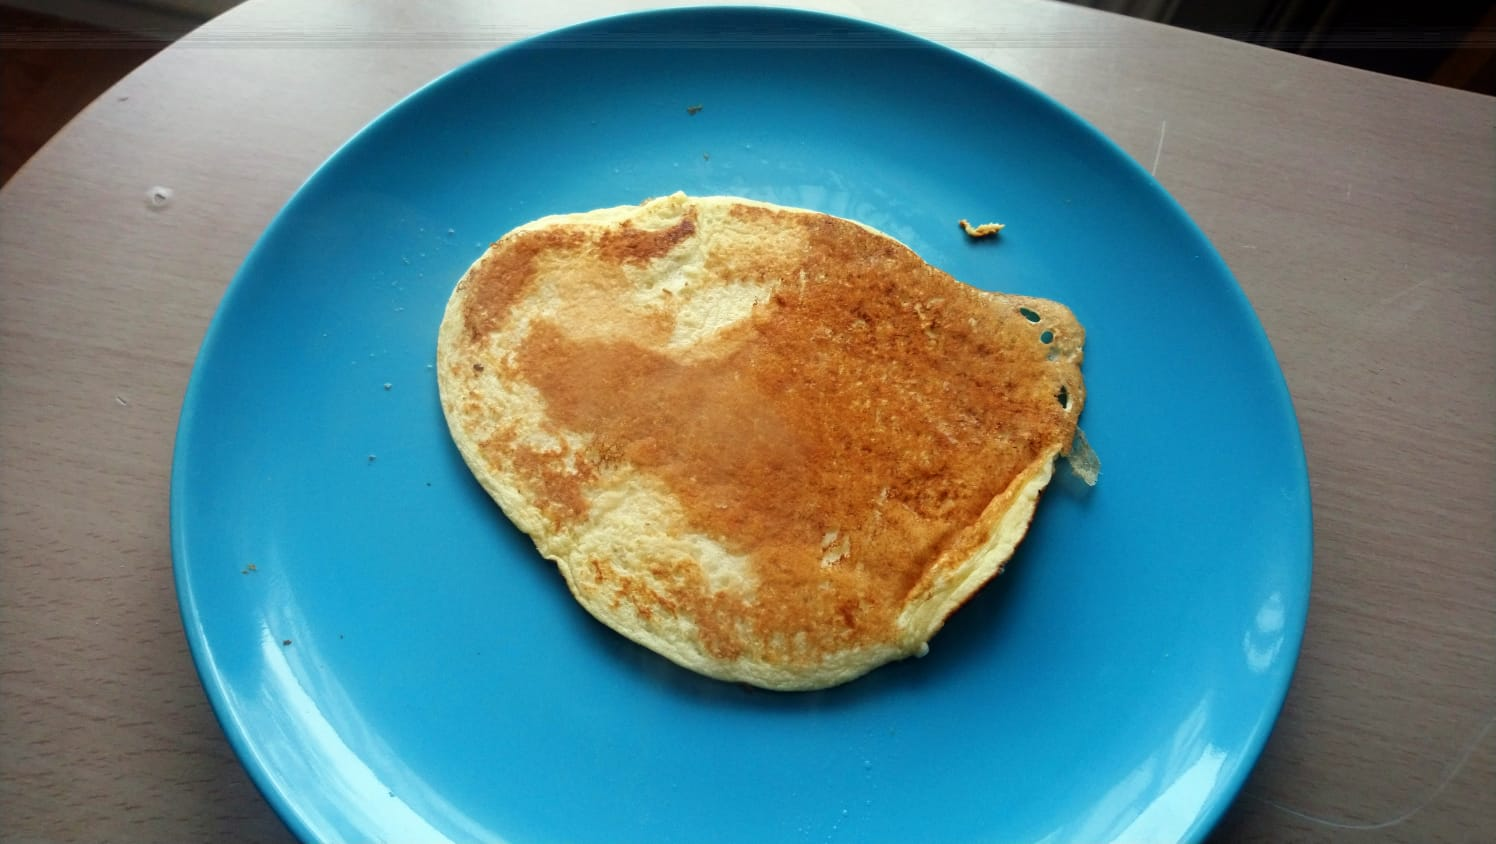
\includegraphics[width=\textwidth]{img/pancakes/pancakes_gebraten.jpg} \cite{pancakes}

\subsection*{How it's done:}

\begin{tabular}{p{15cm}}
	\\
  Separate the eggs and whisk the egg whites with a whisk.\\
  Mix the sugar, milk, egg yolk and pinch of salt.\\
  Sift the flour into the mixture. This makes the dough finer.\\
  Now fold in the beaten egg white slowly and carefully so that it does not disintegrate again.\\
  Heat the oil in a pan. To check, hold the back of a wooden cooking spoon or a wooden stick in the oil. If the oil blows, it's hot enough.\\
  Pour the dough into the pan with a medium ladle.\\
  Brown the pancakes on both sides until golden brown.\\
  Sprinkle with icing sugar and serve hot.
\end{tabular}

\section{\textsc{Pancakes}}

\subsection*{Ingredients:}

\begin{tabular}{p{7.5cm} p{7.5cm}}
	& \\
	\sfrac{1}{4}l milk & 2 eggs \\
	1EL flour & pinch of salt \& sugar \\
  oil for the pan
\end{tabular}

\subsection*{Serving suggestion:}


\includegraphics[width=\textwidth]{img/ph.jpg} \cite{pfannkuchen}

\subsection*{How it's done:}

\begin{tabular}{p{15cm}}
	\\
  Heat the oil in the pan. In the meantime, mix the ingredients properly.\\
  The flour should not form large lumps. If you like, you can sift the flour first.\\
  Pour the dough into the pan with a large ladle.\\
  As soon as the outer edge of the pancakes turns brown, it is time to turn them over.\\
  On the other hand, let it brown and serve.\\
  Dust with icing sugar or cinnamon and you're done.
\end{tabular}

\section{\textsc{Vinaigrette}}

\subsection*{Ingredients for 100ml:}

\begin{tabular}{p{7.5cm} p{7.5cm}}
	& \\
	25ml vinegar & salt, pepper \& sugar \\
	75ml oil & 
\end{tabular}

\subsection*{Serving suggestion:}

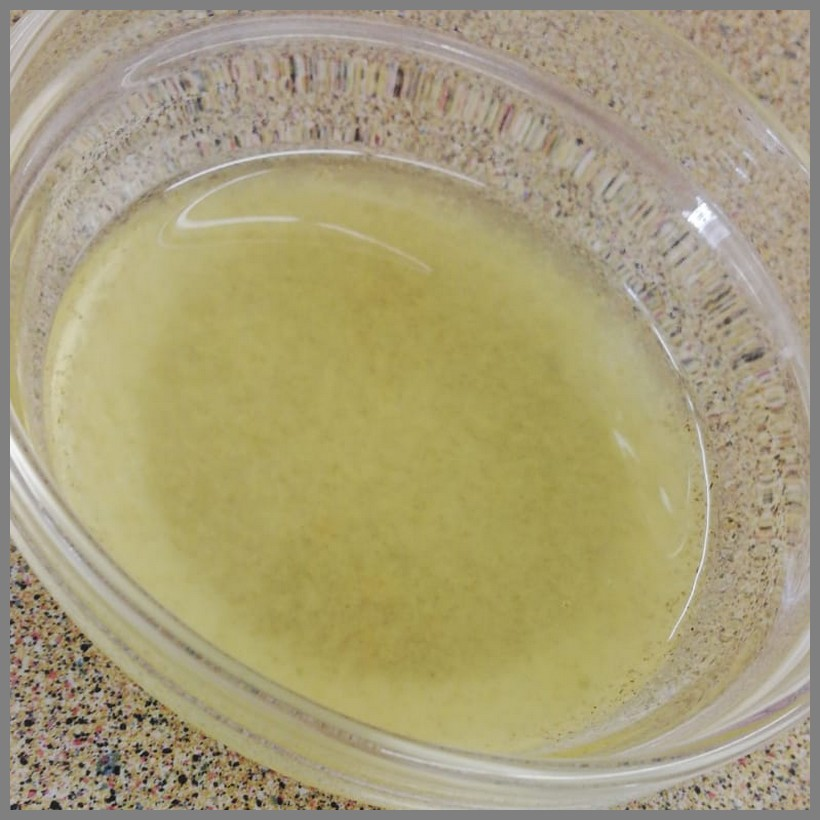
\includegraphics[width=\textwidth]{img/d_vinaigrette.jpeg} \cite{vinaigrette}

\subsection*{How it's done:}

\begin{tabular}{p{15cm}}
	\\
	Dissolve the salt in the vinegar, add the oil.\\
	Season it with pepper and finish it with sugar.\\
	\textbf{Tip:} You can use lemon or lime juice instead of vinegar.\\
	\\
	Suitable for all kinds of salad.
\end{tabular}

\section{\textsc{French dressing}}

\subsection*{Ingredients for 100ml:}

\begin{tabular}{p{7.5cm} p{7.5cm}}
	& \\
	40ml vinegar & french mustard \\
	60ml oil & garlic \\
	salt \& pepper &
\end{tabular}

\subsection*{Serving suggestion:}

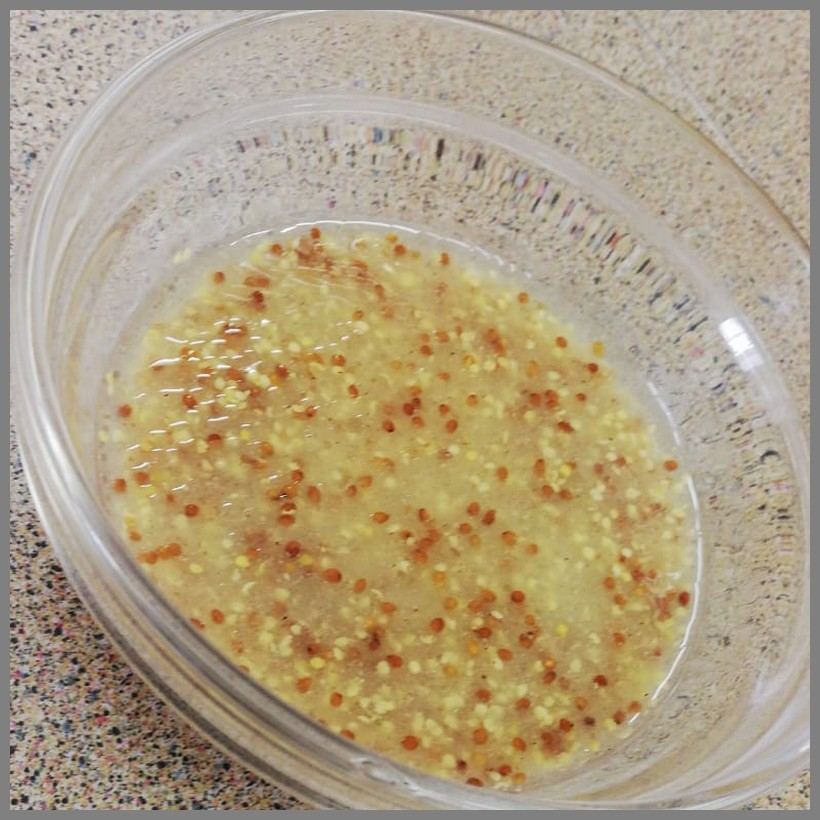
\includegraphics[width=\textwidth]{img/d_french.jpeg} \cite{dfrench}

\subsection*{How it's done:}

\begin{tabular}{p{15cm}}
	\\
	Rub a salad bowl with a half divided clove of garlic.\\
	Add salt, vinegar \& mustard.\\
	Slowly add the oil and stir the dressing.\\
	Season with pepper.\\
	\\
	Suitable for all leaf and vegetable salads.
\end{tabular}

\section{\textsc{Dressing with herbs}}

\subsection*{Ingredients for 100ml:}

\begin{tabular}{p{7.5cm} p{7.5cm}}
	& \\
	40ml vinegar & herbs \\
	60ml oil & shallot \\
	salt \& pepper &
\end{tabular}

\subsection*{Serving suggestion:}

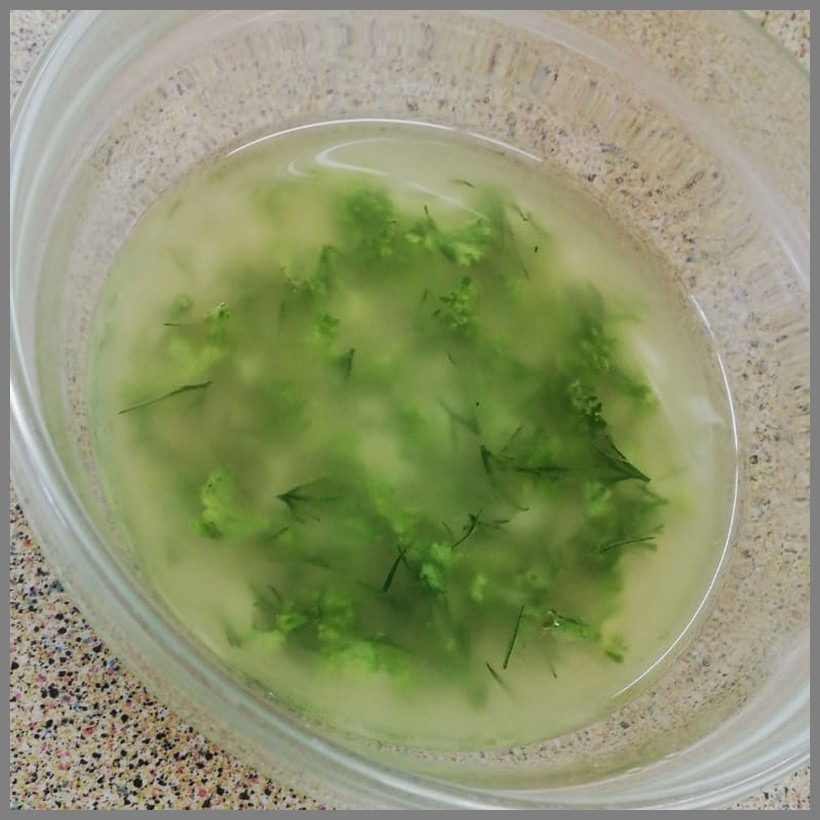
\includegraphics[width=\textwidth]{img/d_krauter.jpeg} \cite{dkrauter}

\subsection*{How it's done:}

\begin{tabular}{p{15cm}}
	\\
	Dissolve the salt in the vinegar, add oil and season it.\\
	Add fresh chopped herbs and julienned shallot.\\
	\\
	Suitable for salads without fruits.
\end{tabular}

\section{\textsc{Dressing with cream}}

\subsection*{Ingredients for 300ml:}

\begin{tabular}{p{7.5cm} p{7.5cm}}
	& \\
	250ml cream & salt, pepper \& sweet paprika \\
	50ml lemon juice & 
\end{tabular}

\subsection*{Serving suggestion:}

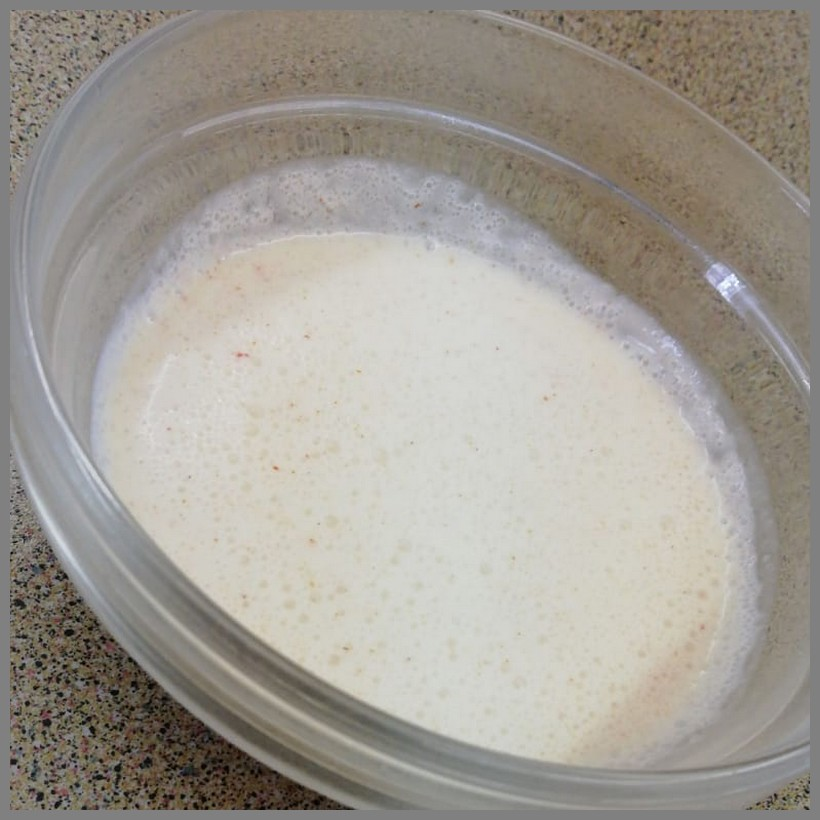
\includegraphics[width=\textwidth]{img/d_sahne.jpeg} \cite{dsahne}

\subsection*{How it's done:}

\begin{tabular}{p{15cm}}
	\\
	Stir the cream with the juice and season it afterwards.\\
	\\
	Suitable for leaf salad, salad with fruits and vegetable salad.
\end{tabular}

\section{\textsc{Dressing with yogurt}}

\subsection*{Ingredients for 300ml:}

\begin{tabular}{p{7.5cm} p{7.5cm}}
	& \\
	250g yogurt & 10ml orange juice \\
	10ml oil & 5ml lemon juice \\
	worcester sauce & salt \& pepper
\end{tabular}

\subsection*{Serving suggestion:}

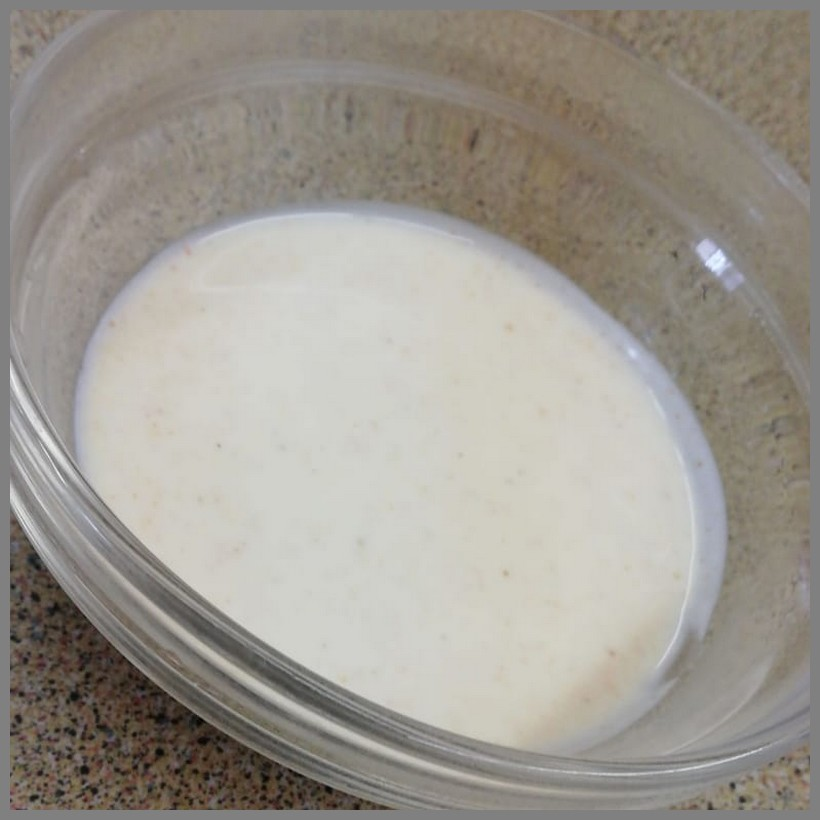
\includegraphics[width=\textwidth]{img/d_joghurt.jpeg} \cite{djoghurt}

\subsection*{How it's done:}

\begin{tabular}{p{15cm}}
	\\
	Stir yogurt, orange juice, lemon juice and a small drop worcester sauce to smooth paste.\\
	Add oil and season with salt and pepper.\\
	\\
	Suitable for all kinds of salad.
\end{tabular}

\section{\textsc{Dressing with cream and dill}}

\subsection*{Ingredients for 300ml:}

\begin{tabular}{p{7.5cm} p{7.5cm}}
	& \\
	250ml sour creame or créme fraîche & 5g chopped dill\\
	50ml lemon or lime juice & salt \& pepper
\end{tabular}

\subsection*{Serving suggestion:}

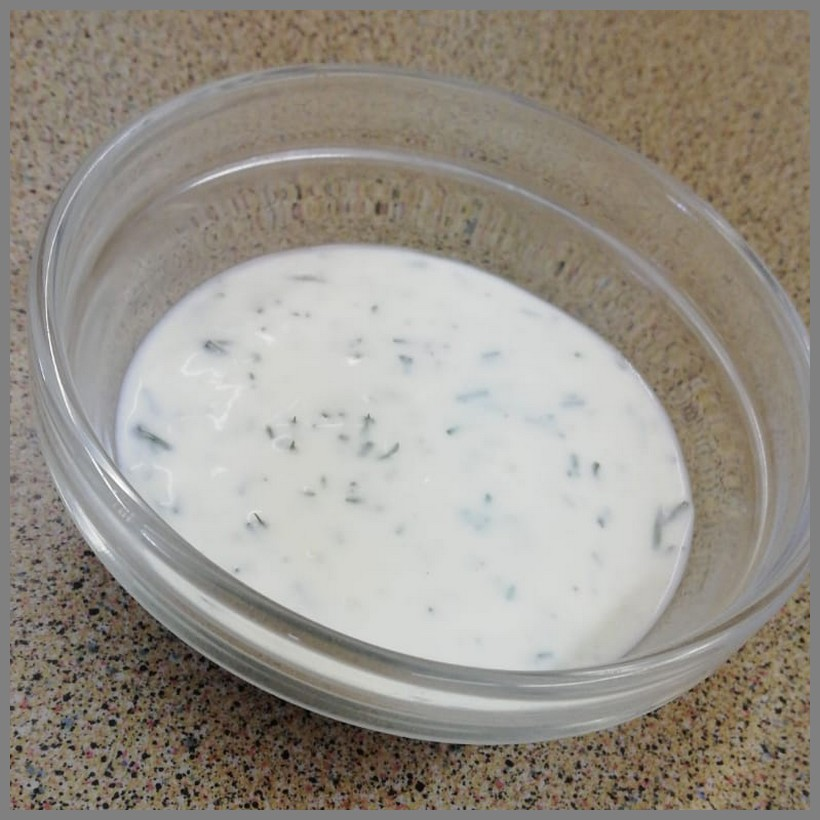
\includegraphics[width=\textwidth]{img/d_dillsahne.jpeg} \cite{dsahnedill}

\subsection*{How it's done:}

\begin{tabular}{p{15cm}}
	\\
	Stir the cream with the juice to a smooth paste.\\
	Add dill and season with salt and pepper.\\
	\\
	Suitable for leaf salad and vegetable salad.
\end{tabular}

\section{\textsc{Cocktail sauce}}

\subsection*{Ingredients for 100ml:}

\begin{tabular}{p{7.5cm} p{7.5cm}}
	& \\
	80g spicy mayonnaise & 5g whipped cream\\
	40g mashed tomato flesh & small drop brandy \\
	1pinch of horseradish & worcester sauce \\
	salt, pepper \& sugar 
\end{tabular}

\subsection*{Serving suggestion:}

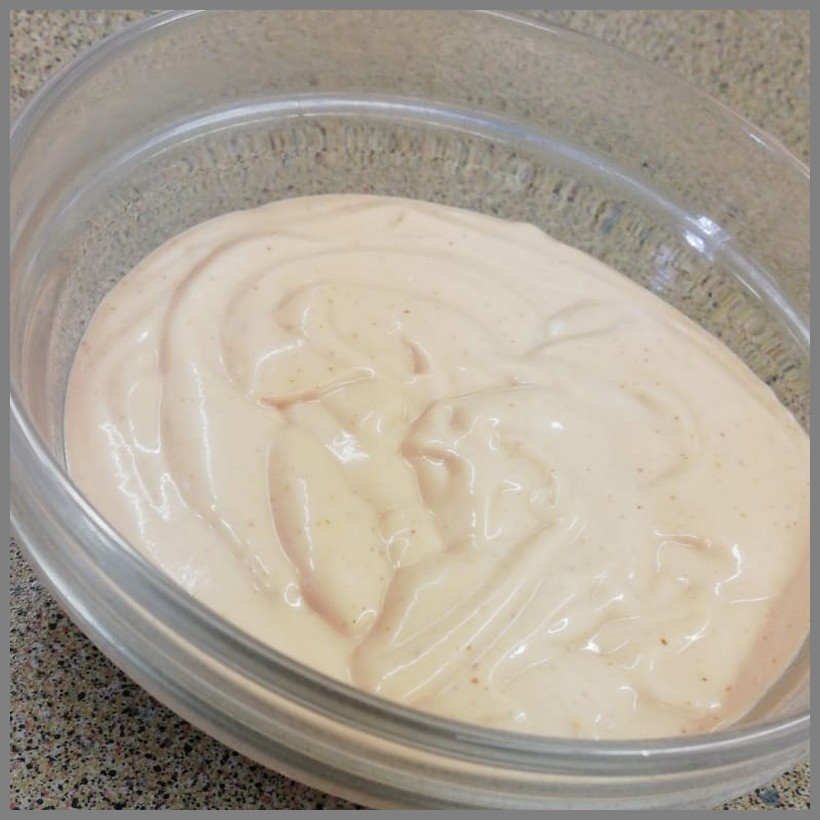
\includegraphics[width=\textwidth]{img/d_cocktail.jpeg} \cite{dcocktail}

\subsection*{How it's done:}

\begin{tabular}{p{15cm}}
	\\
	Stir the mayonnaise with tomato purée to a smooth paste.\\
	Add the cream and season it.\\
	\\
	Suitable for leaf salad and vegetable salad.
\end{tabular}


\newpage
\renewcommand{\refname}{\textsc{References:}}
\begin{thebibliography}{9}
	\bibitem[Side salad]{beilagensalat} Lisa Machoi, 2019
	\bibitem[Raw vegetable salad with apple]{rohkostapfel} Lisa Machoi, 2019
	\bibitem[Coleslaw Salad]{uskrautsalat} Lisa Machoi, 2019
	\bibitem[Fast cucumber salad with sour cream and dill]{gurkensalatdill} Lisa Machoi, 2019
	\bibitem[Cucumber salad]{gurkensalat} Lisa Machoi, 2019
	\bibitem[Spring egg salad]{fruehlingeiersalat} Lisa Machoi, 2019
	\bibitem[Omelette]{omlett} Lisa Machoi, 2019
	\bibitem[Whipped omelette]{omlettwiener} Lisa Machoi, 2019
	\bibitem[Omelette tomo]{omlettomo} Lisa Machoi, 2019
	\bibitem[Fried eggs]{spiegelei} Lisa Machoi, 2019
	\bibitem[Italian fried eggs]{itaspiegelei} Lisa Machoi, 2019
	\bibitem[Scrambled eggs]{ruehrei} Lisa Machoi, 2019
	\bibitem[Scrambled eggs on wholemeal rolls]{ruehreivollkorn} Lisa Machoi, 2019
	\bibitem[Egg in a saucer]{eiimnaepfchen} Lisa Machoi, 2019
	\bibitem[French egg in a saucer]{eiimnaepfchenfranz} Lisa Machoi, 2019
	\bibitem[Poached egg in mustard sauce]{eisenfsosse} Lisa Machoi, 2019
	\bibitem[Spaghetti spinach carbonara with poached egg]{eicorbonara} Lisa Machoi, 2019
	\bibitem[Egg pancakes]{pancakes} Lisa Machoi, 2019
	\bibitem[Pancakes]{pfannkuchen} Lisa Machoi, 2019
	\bibitem[Vinaigrette]{vinaigrette} Lisa Machoi, 2019
	\bibitem[French dressing]{dfrench} Lisa Machoi, 2019
	\bibitem[Dressing with herbs]{dkrauter} Lisa Machoi, 2019
	\bibitem[Dressing with cream]{dsahne} Lisa Machoi, 2019
	\bibitem[Dressing with yogurt]{djoghurt} Lisa Machoi, 2019
	\bibitem[Dressing with dill and cream]{dsahnedill} Lisa Machoi, 2019
	\bibitem[Cocktail sauce]{dcocktail} Lisa Machoi, 2019
\end{thebibliography}
\vspace{1cm}
\begin{center}
	\LaTeX - documents available on\\ \href{https://github.com/lisamachoi/kochprojekt}{\textbf{https://github.com/lisamachoi/kochprojekt}}
	
	\vspace{1cm}
	
	This document is licensed under the\\ \href{https://creativecommons.org/licenses/by-sa/4.0/}{\textbf{Creative Commons Attribution-ShareAlike 4.0 International}}\\
	License.

	\vspace{1cm}

	{\huge\ccbysa}
\end{center}

\end{document}
